\documentclass{beamer}

%\mode<presentation>{
%	\usecolortheme{beaver}
%	\setbeamercovered{transparent}
%}

\usepackage[french]{babel}
\usepackage[utf8]{inputenc}
\usepackage{times}
\usepackage[T1]{fontenc}
\usepackage{graphicx}
\usepackage{xcolor}
\usepackage{verbatim}
\definecolor{bleu1}{RGB}{0,0,128} 
\definecolor{bleu2}{RGB}{0,0,205} 
\definecolor{bleuWRET}{RGB}{67,136,204} 

\title{\textcolor{bleu2}{\textbf{Projet W.R.E.T. (WebRegEfmTool)}}}
\subtitle{\textcolor{bleu1}{Conception d'un projet de recherche}}
\author[]{Arnaud \textsc{Frèche} -- Charlotte \textsc{Héricé} -- Saraï \textsc{Mola} -- \\ Typhaine \textsc{Paysan-Lafosse} -- Joris \textsc{Sansen}}
\institute{Master 2 BioInformatique}
\date{21 février 2013}

\setbeamerfont{author in sidebar}{size=\footnotesize;fg=blue}
\setbeamerfont{title in sidebar}{size=\footnotesize;fg=blue}
\setbeamerfont{section in sidebar}{size=\scriptsize;fg=blue}
\setbeamercolor{palette sidebar secondary}{bg=blue}
\setbeamercolor{author in sidebar}{bg=blue}
\setbeamercolor{title in sidebar}{bg=blue}
\usepackage{pgf}
\pgfdeclareimage[height=96mm,width=10mm]{fond}{fond.png}				% Image de fond
  \setbeamertemplate{background}{\pgfuseimage{fond}}
\logo{}

%\setbeamersize{sidebar width left=0cm}
\setbeamertemplate{navigation symbols}{}


\begin{document}

\frame{\titlepage}
%\frame{\tableofcontents}
\addtobeamertemplate{footline}{\insertframenumber/\inserttotalframenumber}


%%%%%%%%%%%%%%%%%%%%%%%%%%%%%%%%%%
\section*{Introduction}
%%%%%%%%%%%%%%%%%%%%%%%%%%%%%%%%%%

\begin{frame}{\textcolor{bleu2}{\hspace{1cm}Contexte}}
	\begin{columns}
		\begin{column}{7cm}
			\begin{block}{\hspace{0.4cm}Sujet}
				\begin{itemize}
					\item Métabolisme d'une cellule : 
					\begin{itemize}
						\item Transformations moléculaires et énergétiques
						\item Réactions métaboliques
					\end{itemize}
					\item Calculs de modes élémentaires
					\item Quelques logiciels disponibles
				\end{itemize}
			\end{block}
		\end{column}	
		\begin{column}{3.5cm}
			\begin{figure}
				\includegraphics[scale=0.25]{../Images/Rapport/glycolyse-1.png}
				\caption{Exemple d'une partie de la glycolyse}
			\end{figure}
		\end{column}
	\end{columns}
\end{frame}

\begin{frame}{\textcolor{bleu2}{\hspace{1cm}Contexte - RegEfmtool}}
	\begin{center}
		\begin{minipage}[c]{0.9\textwidth}
			\begin{block}{\hspace{0.2cm}Regular Elementary flux mode tool}
				\begin{itemize}
					\item Calcul de modes élémentaires
					\item Environnement UNIX, ligne de commandes
					\item Plusieurs fichiers d'entrée au format \textit{txt}
				\end{itemize}
			\end{block}
			\begin{block}{\hspace{0.2cm}Objectif}
				\begin{itemize}
					\item Interface graphique
					\item Langages Web
				\end{itemize}
			\end{block}
		\end{minipage}
	\end{center}
\end{frame}

\begin{frame}{\textcolor{bleu2}{\hspace{1cm}Interface graphique}}
	\begin{block}{\hspace{0.2cm}WebRegEfmTool}
		\begin{itemize}
			\item Site Web
			\item Utilisation plus conviviale pour \emph{regEfmtool}
			\item Génération les fichiers nécessaires à \emph{regEfmtool}
			\item Création de fichiers fonctionnels au format DAT
			\item Simulations comparées de modes élémentaires
		\end{itemize}
	\end{block}
\end{frame}

%%%%%%%%%%%%%%%%%%%%%%%%%%%%%%%%%%
\section{Création d'un nouveau réseau}
%%%%%%%%%%%%%%%%%%%%%%%%%%%%%%%%%%

\begin{frame}{\textcolor{bleu2}{\hspace{1cm}Création - Fichiers}}
	\begin{figure}[!ht]
		\begin{center}
			\fbox{
   				\begin{minipage}[c]{0.9\textwidth}
  					\includegraphics[width=0.95\textwidth]{../Images/Rapport/create1.png}
				\end{minipage}
			}
			\caption{Page de création d'un nouveau réseau}
			\end{center}
	\end{figure}
	\begin{center}
		\begin{minipage}[c]{0.9\textwidth}
			\begin{block}{\hspace{0.2cm}Initialisation des fichiers}
				\begin{itemize}
					\item Efface fichiers déjà existants
					\item Génère de nouveaux
				\end{itemize}
			\end{block}
		\end{minipage}
	\end{center}
\end{frame}

\begin{frame}{\textcolor{bleu2}{\hspace{1cm}Création - Fichiers}}
	\begin{center}
		\begin{minipage}[c]{0.9\textwidth}
			\begin{block}{\hspace{0.2cm}Fichiers d'entrée nécessaire à \emph{regEfmtool}}
				\begin{itemize}
					\item Réversibilité
					\item Métabolites
					\item Enzymes
					\item Stœchiométrie
					\item Règles des gènes
				\end{itemize}
			\end{block}
		\end{minipage}
	\end{center}
	\begin{figure}[!ht]
		\begin{center}
			\fbox{
   				\begin{minipage}[c]{0.8\textwidth}
  					\includegraphics[width=0.9\textwidth]{../WRET/Diagramme/create2.png}
				\end{minipage}
			}
			\caption{Diagramme de création}
  		\end{center}
	\end{figure}
\end{frame}

\begin{frame}{\textcolor{bleu2}{\hspace{1cm}Création - Fichiers}}
\footnotesize
	\begin{center}
		\begin{minipage}[c]{1\textwidth}
			\begin{block}{\hspace{0.2cm}Réactions et réversibilité}
				\begin{itemize}
					\item Réactions une à une
					\item Syntaxe propre au format \emph{DAT}: \emph{"Pyk : PEP + ADP = Pyr + ATP ."}
					\item Réversibilité via \texttt{radioboutons}
					\item Ordre conservé
				\end{itemize}
			\end{block}
			\begin{block}{\hspace{0.2cm}Noms de réactions, métabolites}
				\begin{itemize}
					\item Parsage liste de réactions
					\item Extraction métabolites
					\item Extraction noms réactions (enzymes)
				\end{itemize}
			\end{block}
			\begin{block}{\hspace{0.2cm}Stœchiométrie}
				\begin{itemize}
					\item Parsage liste de réactions, métabolites
					\item 1 réaction = 1 liste
					\item Matrice = liste de listes
				\end{itemize}
			\end{block}
		\end{minipage}
	\end{center}
\end{frame}

\begin{frame}{\textcolor{bleu2}{\hspace{1cm}Création - Modification et exportation \emph{DAT}}}
\small
	\begin{columns}
		\begin{column}[l]{4cm}
		\begin{block}{\hspace{0.2cm}Modifications}
				\begin{itemize}
					\item Zone de texte
					\item Affichages du réseaux enregistré
					\item Dépendances gérées
				\end{itemize}
			\end{block}
			\begin{block}{\hspace{0.2cm}Exportation au format \emph{DAT}}
				\begin{itemize}
					\item Après création réseau complet
					\item Parsage des métabolites
					\item Choix métabolites externes et internes
				\end{itemize}
			\end{block}
		\end{column}
		\begin{column}[r]{6cm}
			\begin{figure}[!ht]
				\begin{center}
					\fbox{
   						\begin{minipage}[c]{0.8\textwidth}
  							\includegraphics[width=0.9\textwidth]{../Images/Rapport/modif.png}
		 				\end{minipage}
		 			}
					\caption{Zone de modification}
  				\end{center}
			\end{figure}
			\begin{figure}[!ht]
				\begin{center}
					\fbox{
   						\begin{minipage}[c]{0.75\textwidth}
  							\includegraphics[width=0.9\textwidth]{../Images/Rapport/dat2.png}
						\end{minipage}
					}
					\caption{Choix des métabolites internes et externes}
  				\end{center}
			\end{figure}
		\end{column}
	\end{columns}
\end{frame}

%%%%%%%%%%%%%%%%%%%%%%%%%%%%%%%%%%
\section{Règles des gènes}
%%%%%%%%%%%%%%%%%%%%%%%%%%%%%%%%%%

\begin{frame}
	\frametitle{\hspace{1cm}\textcolor{bleu2}{\secname}}
	\begin{center}
		\begin{minipage}[c]{0.9\textwidth}
			\begin{block}{\hspace{0.2cm}Utilité}
				Élimination modes élémentaires non possibles dans réseau chez organisme vivant
			\end{block}
			\begin{block}{\hspace{0.2cm}États d'une réaction}
				\begin{itemize}
					\item 1-active (R=1)
					\item 0-active (R=0)
					\item full-active (R=f)
				\end{itemize}
			\end{block}
		\end{minipage}
	\end{center}
\end{frame}

\begin{frame}
	\frametitle{\hspace{1cm}\textcolor{bleu2}{\secname}}
	\begin{figure}[!ht]
		\begin{center}
			\fbox{
   		 		\begin{minipage}[c]{0.98\textwidth}
  					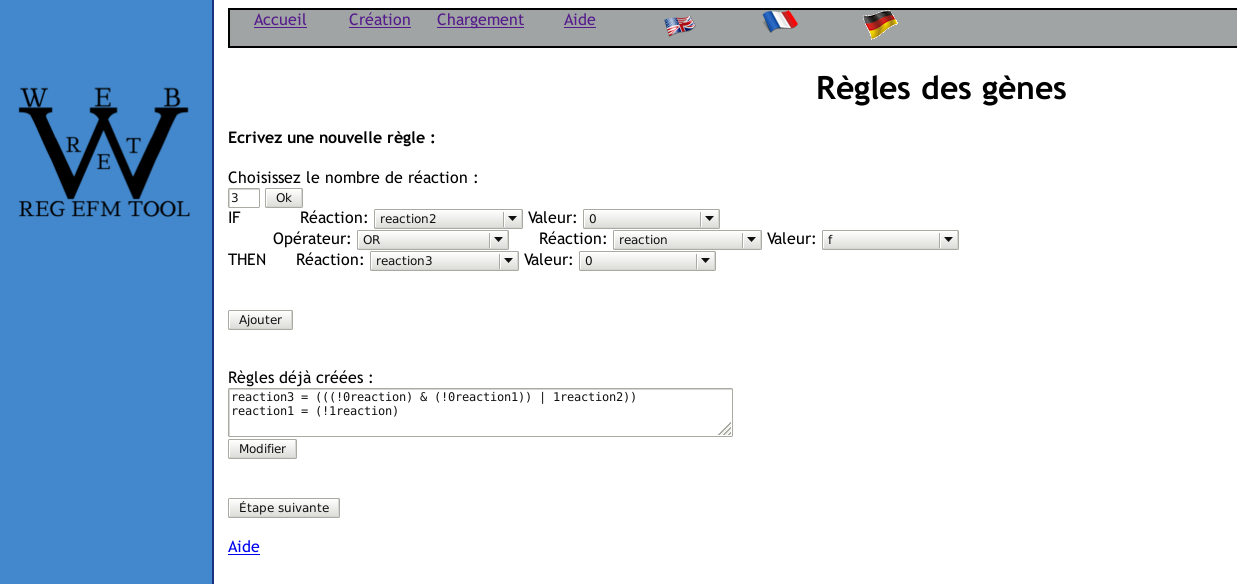
\includegraphics[scale=0.24]{../Images/Rapport/generules.png}  
				\end{minipage}
			}
			\caption{Page de création des règles des gènes}
  		\end{center}	
	\end{figure}
\end{frame}

\begin{frame}
	\frametitle{\hspace{1cm}\textcolor{bleu2}{\secname}}
	\begin{figure}[!ht]
		\begin{center}
			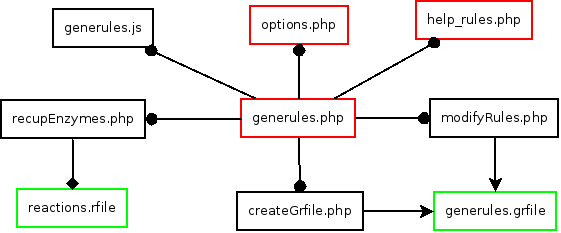
\includegraphics[scale=0.5]{../WRET/Diagramme/generules.png}  
			\caption{Diagramme de création des règles}
  		\end{center}	
	\end{figure}
\end{frame}

\begin{frame}[fragile]
	\frametitle{\hspace{1cm}\textcolor{bleu2}{\secname}}
	\begin{block}{\hspace{0.2cm}Création des règles}
		\hspace{1cm}
		\begin{center}
			\begin{tabular}{|c|c|c|}
				\hline
				Valeur R & THEN=0 & THEN=1\\ \hline
				0 & !0R & 0R\\ \hline
				1 & !1R & 1R\\ \hline
				f & !fR & fR\\ \hline
			\end{tabular}
		\end{center}
	\end{block}
	\begin{block}{\hspace{0.2cm}Exemple}
		\begin{center}
			\begin{minipage}[c]{0.8\textwidth}
				\hspace{2cm}
				\begin{verbatim}
					IF réaction: R1 valeur: 1
					Opérateur: AND réaction: R2 valeur: 0
					Opérateur: OR réaction: R3 valeur: 0
					THEN réaction: R4 valeur: 0

					R4 = (!((1R1 & (!0R2)) | (!0R3))
				\end{verbatim}
			\end{minipage}
		\end{center}
	\end{block}
\end{frame}

%%%%%%%%%%%%%%%%%%%%%%%%%%%%%%%%%%
\section{Choix des options de lancement}
%%%%%%%%%%%%%%%%%%%%%%%%%%%%%%%%%%

\begin{frame}{\textcolor{bleu2}{\hspace{1cm}Options de lancement - Choix}}
	\begin{figure}
		\begin{center}
			\fbox{
	 			\begin{minipage}[c]{0.95\textwidth}
					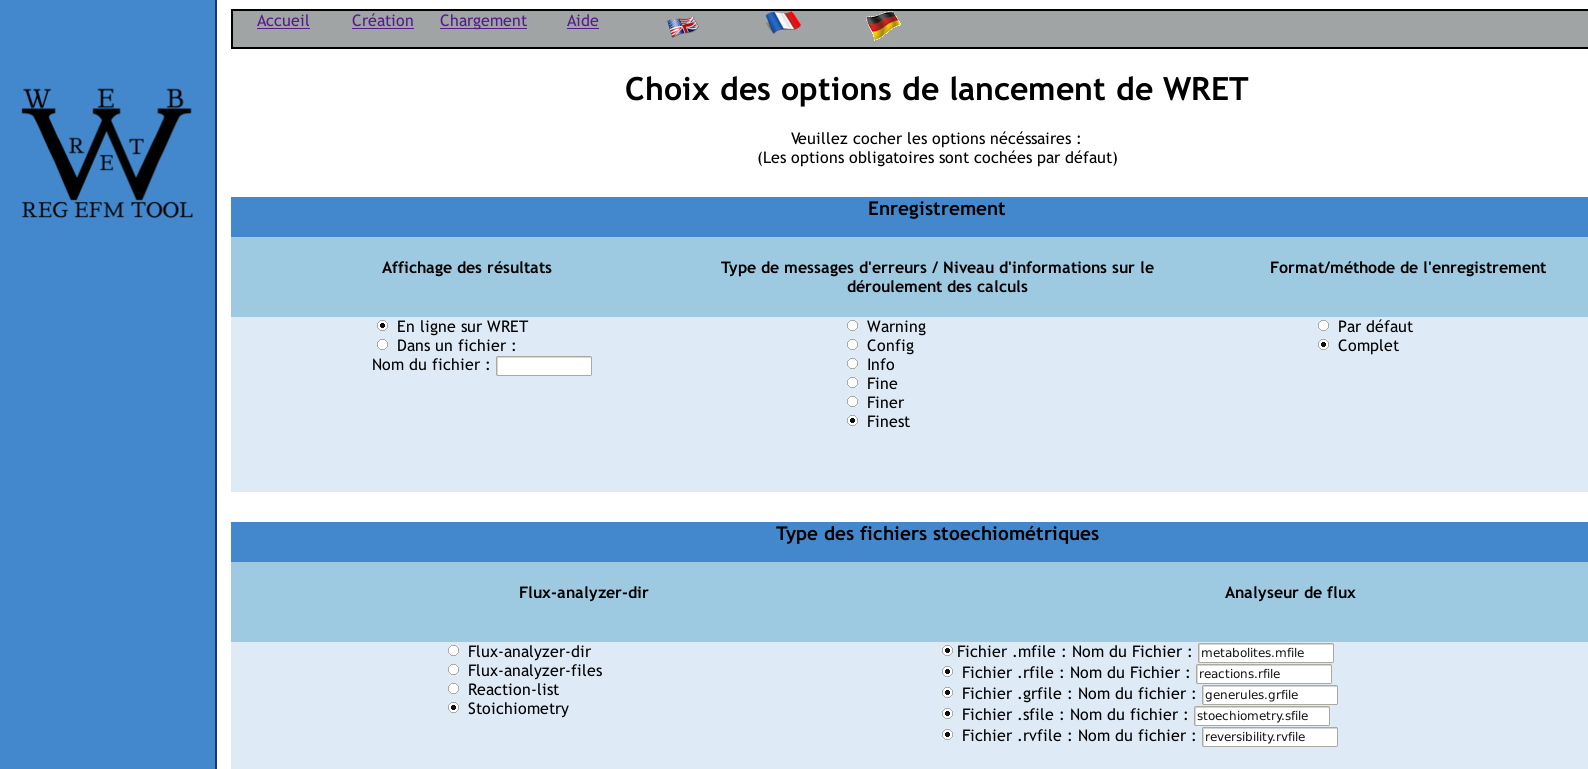
\includegraphics[width=10cm]{../Images/Rapport/options.png}
				\end{minipage}
			}	
			\caption{Partie de la page du choix des options}
		\end{center}
	\end{figure}
\end{frame}

\begin{frame}[fragile]{\textcolor{bleu2}{\hspace{1cm}Options de lancement - Choix}}
	\begin{block}{\hspace{0.2cm}Choix des paramètres de la commande}
		\begin{itemize}
			\item \texttt{radioboutons} et zones de texte dans un formulaire
			\item Paramètre de la commande dans l'attribut \textit{value}
			\item Attribut \textit{name} identique pour les \texttt{radioboutons} d'une même section $\rightarrow$ un seul coché
			\item Paramètres par défaut pré-cochés avec l'attribut \textit{checked="checked"}
		\end{itemize}
	\end{block}
\end{frame}

\begin{frame}[fragile]{\textcolor{bleu2}{\hspace{1cm}Options de lancement - Choix}}
	\begin{figure}
		\begin{center}
			\fbox{
	 			\begin{minipage}[c]{0.4\textwidth}
					
\includegraphics[width=4cm]{../Images/Rapport/options-1.png}
				\end{minipage}
			}	
			\caption{Exemple}
		\end{center}
	\end{figure}
	\scriptsize
	\begin{center}
		\begin{minipage}[c]{0.9\textwidth}
			\begin{verbatim}
				<input type="radio" name="choix1" value="log console"
				 checked="checked">
			\end{verbatim}
			\begin{verbatim}
				<input type="radio" name="choix1" 	value="log file">
				<input type="text" name="log_nomFichier" 	size="10" id="texte1">
			\end{verbatim}
		\end{minipage}
	\end{center}
\end{frame}

\begin{frame}{\textcolor{bleu2}{\hspace{1cm}Options de lancement - Récupération}}
	\begin{figure}
		\begin{center}
			\fbox{
	 			\begin{minipage}[c]{0.6\textwidth}
					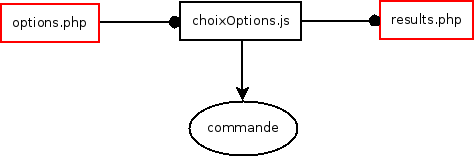
\includegraphics[width=6cm]{../WRET/Diagramme/options.png}
				\end{minipage}
			}	
			\caption{Diagramme d'organisation pour les options}
		\end{center}
	\end{figure}
	\begin{block}{\hspace{0.2cm}JavaScript pour}
		\begin{itemize}
			\item Récupérer l'attribut \textit{value} 
			\item Générer la commande de lancement 
			\item Commande $\rightarrow$ cookie
		\end{itemize}
	\end{block}
\end{frame}

%%%%%%%%%%%%%%%%%%%%%%%%%%%%%%%%%%
\section{Chargement}
%%%%%%%%%%%%%%%%%%%%%%%%%%%%%%%%%%

\begin{frame}[fragile]{\textcolor{bleu2}{\hspace{1cm}Chargement}}
	\begin{center}
		\begin{minipage}[c]{0.9\textwidth}
			\begin{block}{\hspace{0.2cm}But}
 				Charger les fichiers d'un réseau pré-existant
 			\end{block}
 		\end{minipage}
 	\end{center}
	\begin{figure}
		\begin{center}
			\fbox{
				\begin{minipage}[c]{0.95\textwidth}
					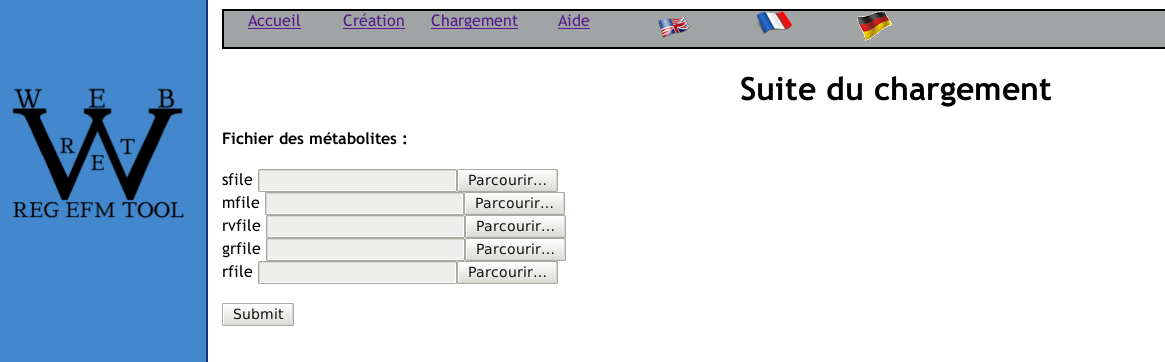
\includegraphics[scale=0.25]{../Images/Rapport/chargement1.png}
				\end{minipage}
			}	
			\caption{Page de chargement des fichiers}
		\end{center}
	\end{figure}
\end{frame}

\begin{frame}[fragile]{\textcolor{bleu2}{\hspace{1cm}Chargement}}
	\begin{figure}
		\begin{center}
			\fbox{
				\begin{minipage}[c]{0.95\textwidth}
					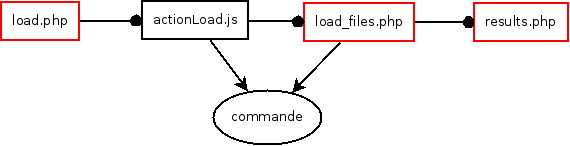
\includegraphics[scale=0.5]{../WRET/Diagramme/load.png}
				\end{minipage}
			}	
			\caption{Diagramme d'organisation pour le chargement}
		\end{center}
	\end{figure}
	\begin{itemize}
		\item \textbf{Récupération} des données :
		\begin{itemize}
			\item Une fonction PHP copie les fichiers dans le répertoire courant
			 \item Utilisation de la fonction PHP {\footnotesize\texttt{move\_uploaded\_file()}}
		\end{itemize}
		\item \textbf{Compléter} la commande générée
	\end{itemize}
\end{frame}

%%%%%%%%%%%%%%%%%%%%%%%%%%%%%%%%%%
\section{Résultats}
%%%%%%%%%%%%%%%%%%%%%%%%%%%%%%%%%%

\begin{frame}{\textcolor{bleu2}{\hspace{1cm} Résultats}}
	\begin{figure}
		\begin{center}
			\fbox{
				\begin{minipage}[c]{0.98\textwidth}
					\includegraphics[scale=0.30]{../Images/Rapport/results_all.png}
				\end{minipage}
			}	
			\caption{Page d'affichage des résultats}
		\end{center}
	\end{figure}
	\begin{itemize}
		\item \textbf{Exécution} de la commande par une fonction PHP {\footnotesize \texttt{shell\_exec()}}
		\item \textbf{Récupération} des résultats et \textbf{Parsage}
	\end{itemize}
\end{frame}

\begin{frame}{\textcolor{bleu2}{\hspace{1cm}Résultats}}
\begin{figure}
		\begin{center}
			\fbox{
				\begin{minipage}[c]{0.98\textwidth}
					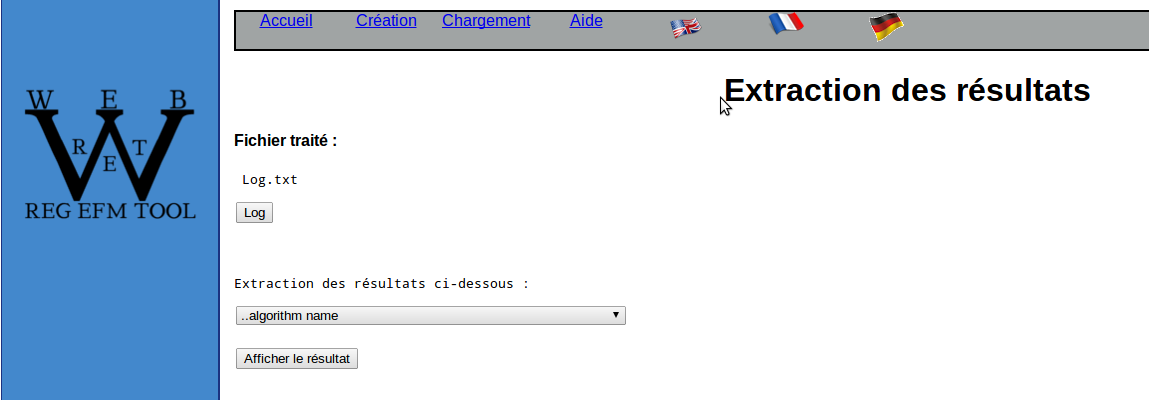
\includegraphics[scale=0.26]{../Images/Rapport/extractionResultat.png}
				\end{minipage}
			}	
			\caption{Page d'extraction des résultats}
		\end{center}
	\end{figure}
	\begin{block}{\hspace{0.2cm}Affichage des Résultats}
		\begin{itemize}
			\item En fonction de la session : comparaison ou non
			\item Possibilité d'afficher le \textit{log} complet ou sélection d'un mot-clé
		\end{itemize}
	\end{block}
\end{frame}

%%%%%%%%%%%%%%%%%%%%%%%%%%%%%%%%%%
\section{Ergonomie de l'interface}
%%%%%%%%%%%%%%%%%%%%%%%%%%%%%%%%%%

\begin{frame}{\textcolor{bleu2}{\hspace{1cm} Ergonomie}}
	\begin{figure}
		\begin{center}
			\fbox{
	 			\begin{minipage}[c]{1.02\textwidth}
					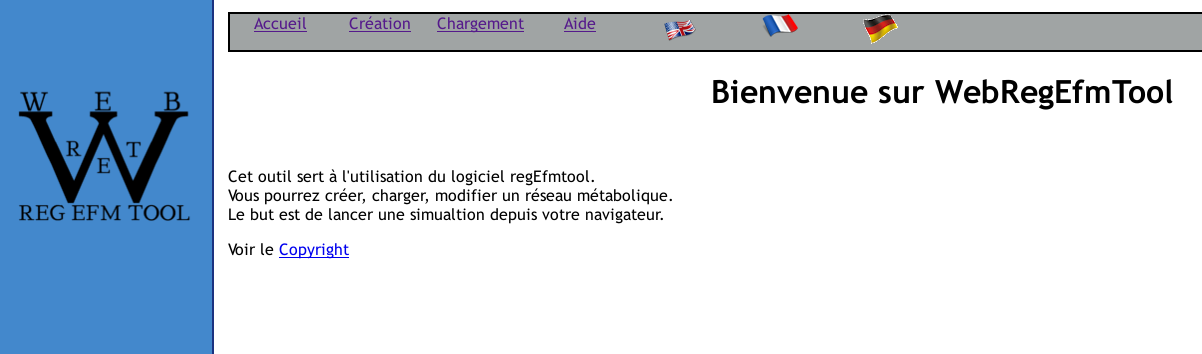
\includegraphics[width=11cm]{../Images/Rapport/pageAccueil.png}
				\end{minipage}
			}	
			\caption{Page d'accueil}
		\end{center}
	\end{figure}
\end{frame}

\begin{frame}{\textcolor{bleu2}{\hspace{1cm} Ergonomie - Mise en page}}
	\begin{figure}
		\begin{center}
			\fbox{
	 			\begin{minipage}[c]{1.02\textwidth}
					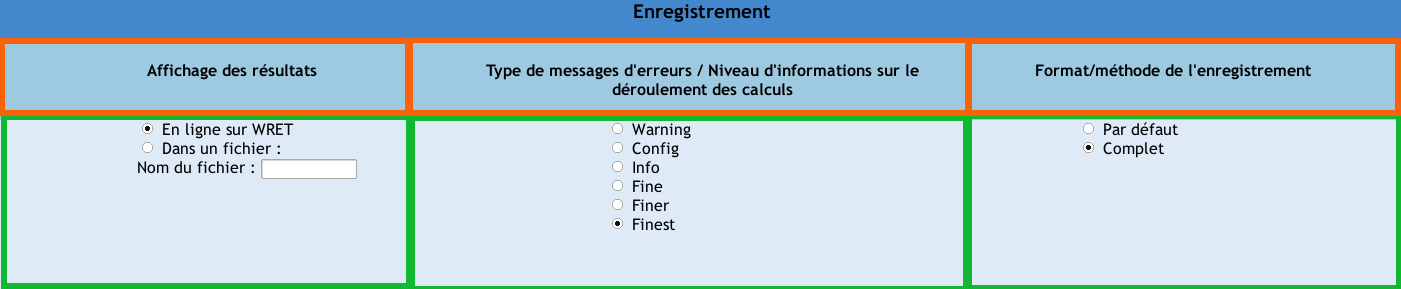
\includegraphics[width=11cm]{../Images/Rapport/options-2.png}
				\end{minipage}
			}	
			\caption{Exemple d'organisation dans la page}
		\end{center}
	\end{figure}
	\hspace{0.2cm}Organisation par \texttt{<div>} :
	\begin{itemize}
		\item \textcolor{blue}{div part} 
		\item \textcolor{orange}{div subPart}
		\item \textcolor{green}{div buttons}
	\end{itemize}
\end{frame}

\begin{frame}[fragile]{\textcolor{bleu2}{\hspace{1cm} Ergonomie - Langues}}
	\begin{figure}
		\begin{center}
			\fbox{
	 			\begin{minipage}[c]{0.8\textwidth}
					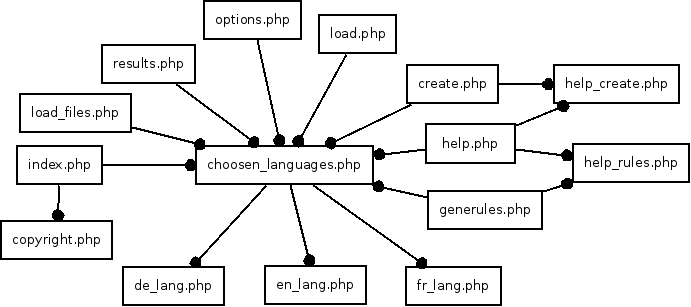
\includegraphics[width=8cm]{../WRET/Diagramme/langues.png}
				\end{minipage}
			}	
			\caption{Diagramme d'organisation pour le changement de langue}
		\end{center}
	\end{figure}
	\begin{block}{\hspace{0.2cm}Exemple du titre de la page d'accueil}
		\begin{center}
			\begin{minipage}[c]{0.9\textwidth}
				\begin{verbatim}
					<?php echo TXT\_SITE\_TITLE; ?>
				\end{verbatim}
				\scriptsize
				\begin{verbatim}
					define('TXT_SITE_TITLE', "Page d'accueil de WebRegEfmTool");
					define('TXT_SITE_TITLE', "Homepage of WebRegEfmTool");
					define('TXT_SITE_TITLE', "Starseite von WebRegEfmTool");
				\end{verbatim}
			\end{minipage}
		\end{center}
	\end{block}
\end{frame}

%%%%%%%%%%%%%%%%%%%%%%%%%%%%%%%%%%
\section{Difficultés et améliorations}
%%%%%%%%%%%%%%%%%%%%%%%%%%%%%%%%%%

\begin{frame}{\textcolor{bleu2}{\hspace{1cm}Difficultés et améliorations}}
	\begin{block}{\hspace{0.2cm}Difficultés}
		\begin{itemize}
			\item Navigateur :
			\begin{itemize}
				\item Fonction \texttt{move\_uploaded\_file()}
				\item Récupération des fichiers \texttt{\$\_FILES}
			\end{itemize}
			\item Affichage des résultats
			\item Configuration du serveur Web
		\end{itemize}
	\end{block}
	\begin{block}{\hspace{0.2cm}Améliorations}
		\begin{itemize}
			\item Ajout et amélioration de fonctionnalités (ex: édition)
			\item Intégrer d'autres logiciels tels que METATOOL
		\end{itemize}
	\end{block}
\end{frame}

%%%%%%%%%%%%%%%%%%%%%%%%%%%%%%%%%%
\section*{Conclusion}
%%%%%%%%%%%%%%%%%%%%%%%%%%%%%%%%%%

\begin{frame}{\textcolor{bleu2}{\hspace{1cm}Conclusion}}
	\begin{itemize}
	\item Réalisation d'une interface graphique pour le logiciel de calculs de modes élémentaires \emph{regEfmtool}
	\item Familiarisation avec les langages propres aux communications et protocoles Web
	\end{itemize}
\end{frame}

\begin{frame}{}
	\begin{center}
		\textcolor{bleu2}{\hspace{1cm}Merci de votre attention}
	\end{center}
\end{frame}

\end{document}

%\centering
%  \includegraphics[width=10cm]{demo-manyclients}

%\begin{frame}
%\begin{columns}
%		\begin{column}{6cm}
%			\begin{itemize}
%			\item Micrographies de complexes protéiques
%			\item Utilisation du logiciel ImageJ
%			\item Sélection manuelle fastidieuse 
%				\begin{itemize}
%				\item Chronophage
%				\item Accapare un membre de l'équipe	
%				\item Répétitive
%				\end{itemize}
%			\end{itemize}
%		\end{column}	
%		\begin{column}{6cm}
%			\begin{figure}
%				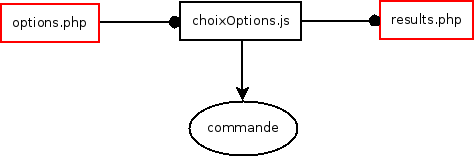
\includegraphics[scale=0.3]{../WRET/Diagramme/options.png}
%		
%			Exemple de micrographie
%			\end{figure}
%		\end{column}
%	\end{columns}
%\end{frame}